\section{Medical Imaging}

\from{HIPS begin}
\subsection{List-mode OSEM (HIPS)}

\emph{List-Mode Ordered Subset Expectation Maximization} (list-mode OSEM) is a time-intensive, production-quality algorithm from a real-world application in medical image reconstruction.
It is used to reconstruct three-dimensional images from huge sets of so-called \emph{events} recorded in \emph{positron emission tomography} (PET).
Each event represents a \emph{line of response} (LOR) which intersects the scanned volume.
A simplified sequential implementation of list-mode OSEM is shown in Listing~\ref{lst:lmosem_seq}.
The algorithm splits the events into \emph{subsets} which are processed iteratively:
All LORs of a subset's events and their corresponding intersection \emph{paths} are computed and merged into an \emph{error image} which is merged with the reconstruction image, thus refining a \emph{reconstruction image} in each iteration.

\begin{lstlisting}[%
caption={Sequential implementation of list-mode OSEM.},%
float=bp,%
label={lst:lmosem_seq}]
for	(l = 0; l < num_subsets; l++) {
	/* read subset from file */
	events = read_events();
	/* compute error image c */
	for	(i = 0; i < num_events; i++) {
		/* compute path of LOR */
		path = compute_path(events[i]);
		/* compute error */
		for	(fp = 0, m = 0; m<path_len; m++)
			fp += f[path[m].coord] * path[m].len;
		/* add path to error image */
		for (m = 0; m<path_len; m++)
			c[path[m].coord] += path[m].len / fp;
	}
	/* update reconstruction image f */
	for	(j = 0; j < image_size; j++)
		if (c[j] > 0.0) f[j] *= c[j];	}
\end{lstlisting}

In a parallel implementation of list-mode OSEM, the loops for calculating the error image ($c$) and for updating the reconstruction image ($f$) can be parallelized.

\subsubsection{Programming effort}

We develop implementations of list-mode OSEM using OpenCL and SkelCL; a CUDA-based implementation using multiple GPUs has already been implemented~\cite{ScVG-08}.
Both, CUDA and OpenCL, require us to add a considerable amount of boilerplate code for running a kernel on multiple GPUs, in particular for uploading and downloading data to and from the GPUs.
In CUDA, we have to create one CPU thread for each device to be managed.
This introduces the additional challenge of multi-threaded programming, including the need of thread synchronization.

\begin{lstlisting}[%
caption={Implementation of list-mode OSEM in SkelCL.},%
float=tbp,%
label={lst:lmosem_skelcl}]
for (l = 0; l < num_subsets; l++) {
	// read events from file
	Vector<Event> events(read_events());
	
	// distribute events to devices
	events.setDistribution(
		Distribution::block);
	// copy reconstruction (f) and error image (c) to all devices
	f.setDistribution(Distribution::copy);
	c.setDistribution(Distribution::copy);
	
	// prepare arguments of error image computation
	SkelCL::Arguments arguments;
	arguments.push(events);
	arguments.push(events.size());
	arguments.push(paths); // memory for paths
	arguments.push(f);
	arguments.push(c);
	
	// compute error image (map skeleton)
	compute_c(index, arguments);
	
	// signal modification of error image
	c.dataOnDevicesModified();
	// distribute reconstruction image to  all devices
	f.setDistribution(Distribution::block);
	// reduce (element-wise add) all copies of error image; re-distribute to all devices after reduction
	c.setDistribution(Distribution::block, add);
	
	// update reconstruction image (zip skeleton)
	update(f, c, f);	}
\end{lstlisting}

With SkelCL, we use the \texttt{Vector} class and the \texttt{Map} and \texttt{Zip} skeletons to implement list-mode OSEM (see Listing~\ref{lst:lmosem_skelcl}).
The events of a subset, as well as the error image and the reconstruction image are stored in a SkelCL \texttt{Vector}.
Thus, we can easily distribute subsets across all GPUs and copy both images to all devices.
We use a \texttt{Map} skeleton to implement the computation of the error image.
However, we must not compute too many paths in parallel to avoid excessive memory consumption.
Therefore, the input of the \texttt{Map} skeleton is not a subset, but rather a vector of 512 indices.
These indices refer to disjoint sub-subsets of events, each of which is processed within a single kernel instance on the GPUs.
For each event, this kernel performs the same steps as the first inner loop in the sequential implementation.
The reconstruction and the error image, as well as the events, are passed to the \texttt{Map} skeleton as additional arguments.
The skeleton produces no result, but updates the error image by side-effect.
Therefore, the error image has to be marked as ``modified on the device'' after executing the \texttt{Map} skeleton.

So far, separate copies of the error image have been used on all GPUs.
To obtain the final error image, we have to merge all copies into a single image.
Afterwards, the final error image and the reconstruction image are distributed across all GPUs, such that each device processes a part of these images.
In SkelCL, the aforementioned data movement is easily achieved by changing the kind of distribution of the vectors that contain this data.
A \texttt{Zip} skeleton is used to implement the update of the reconstruction image, taking the distributed images as input.
The kernel function of this skeleton resembles the body of the second inner loop of the sequential implementation.

The parallelization using SkelCL is quite similar to our CUDA- and OpenCL-based implementations.
However, when using SkelCL's vector data type, we avoid additional programming effort to implement data transfer between host and GPU or between multiple GPUs, and we obtain a multi-GPU-ready implementation of list-mode OSEM for free.
The SkelCL-based implementation is the shortest with 232 lines of code (kernel function: 200~lines, host program: 32~lines).
The CUDA- and OpenCL-based implementations are considerably longer with 329 (199, 130), or even 436 lines of code (193, 243), respectively (see Figure~\ref{fig:lmosem_results}).


\subsubsection{Performance experiments}

We tested our implementations of list-mode OSEM using a typical data set of about $10^7$ events for $150\times 150\times 280$ PET image.
The data set is split into 10 equally sized subsets.
We measured the average runtime of processing all subsets.
Figure~\ref{fig:lmosem_results} shows the runtime of our three implementations of list-mode OSEM using one, two, and four GPUs.

\begin{figure}[tbp]
	\centering
	\label{fig:lmosem_runtime}%
	\label{fig:lmosem_speedup}%
	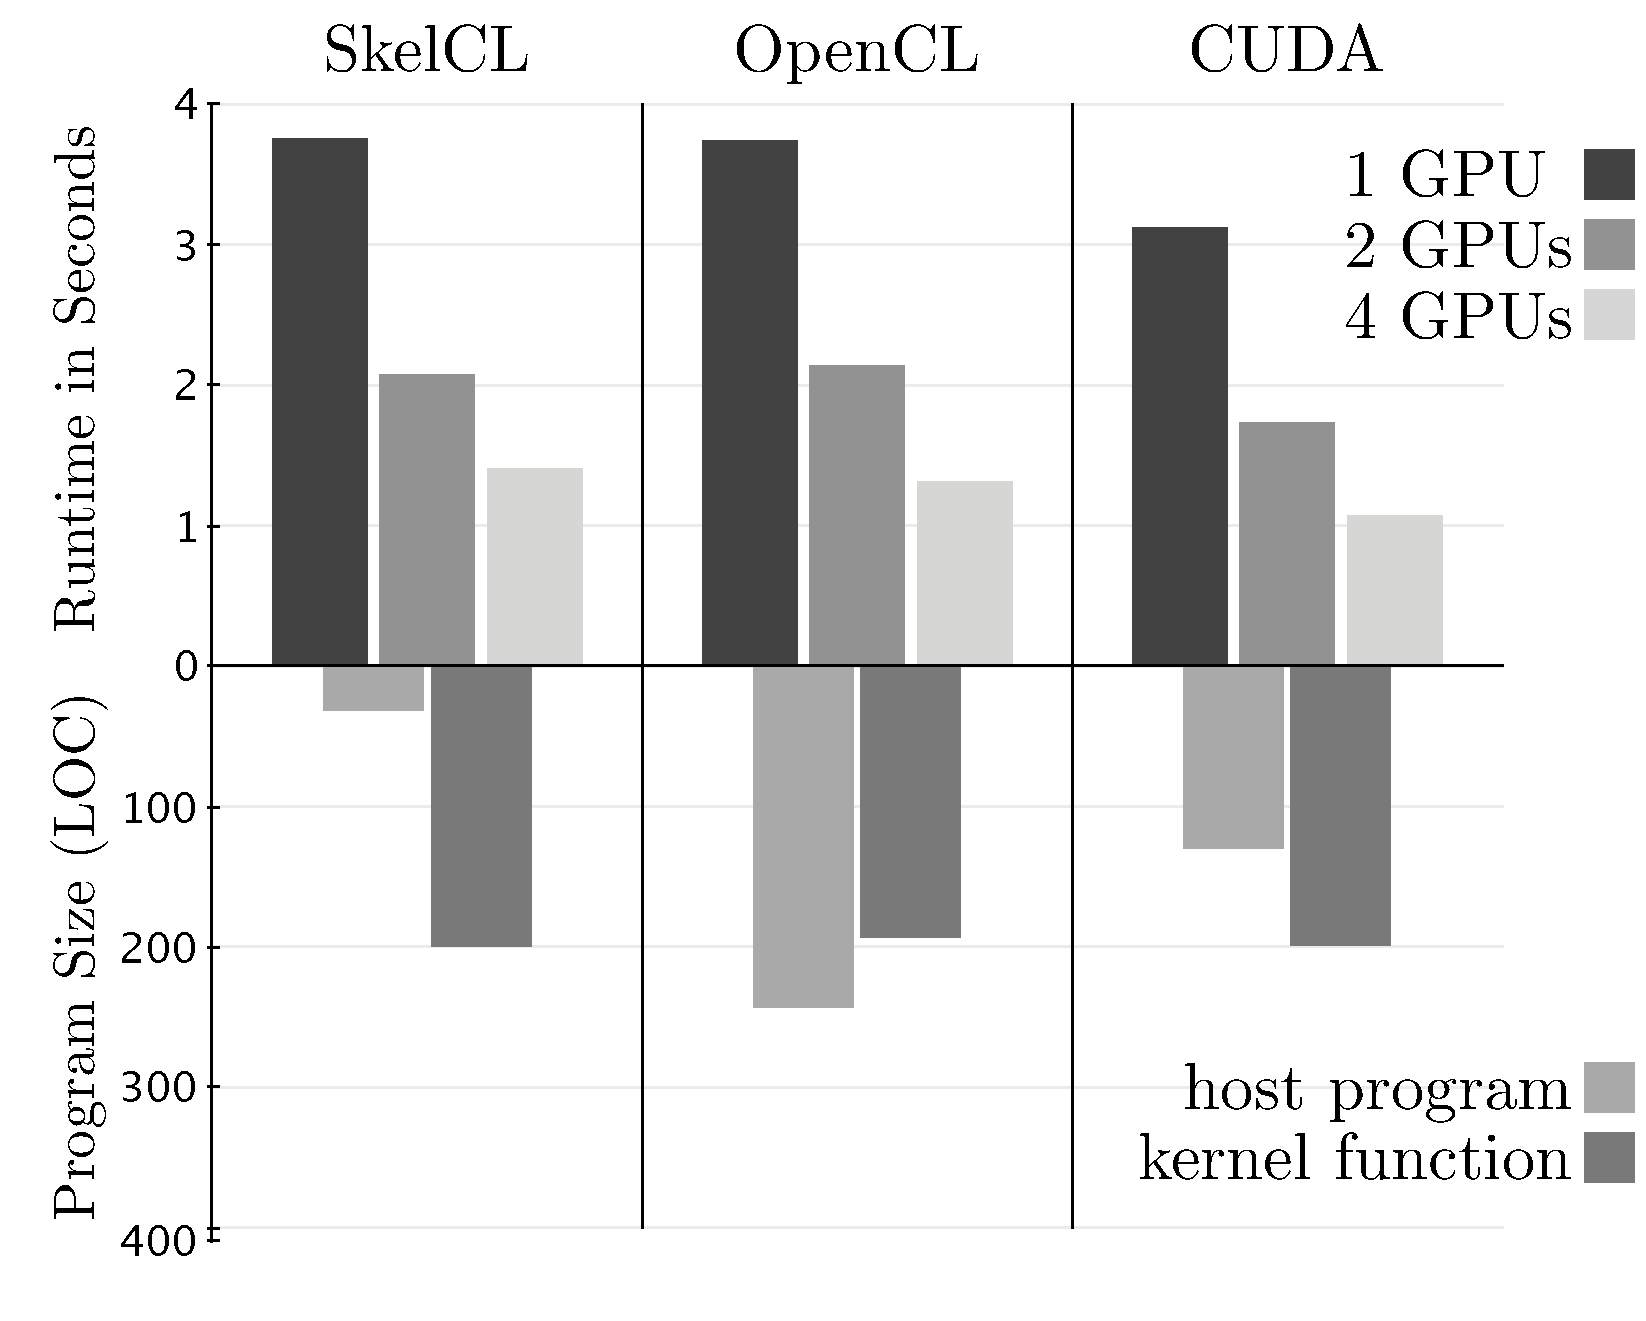
\includegraphics[width=0.42\textwidth]{HIPS/ChartLmosem}
	\caption{Runtime and program size of parallel list-mode OSEM using CUDA, OpenCL, and SkelCL.}
	\label{fig:lmosem_results}
\end{figure}

Running on a single GPU, the CUDA-based implementation (3.03 seconds) outperforms the ones based on OpenCL and SkelCL (3.66 seconds each) by about 20\%.
These relative performane differences also hold for using two GPUs, with only negligible overhead of SkelCL compared to OpenCL.
With four GPUs, the CUDA-based implementation again is faster than the SkelCL- (23\%) and OpenCL-based (17\%) implementations.
SkelCL provides a speedup of 3.1, while OpenCL and CUDA provide speedups of 3.24 and 3.15 respectively.
On four GPUs the SkelCL code runs 2.56 times faster than the CUDA on one GPU.

The SkelCL-based implementation only introduces a moderate overhead of less than 5\% as compared to OpenCL.
Since the OpenCL-based implementation requires a lot of low-level boilerplate code (over 100 lines of code only for initialization), the SkelCL-based implementation clearly provides a higher level of programming.
Especially, the additional argument feature and the data distributions are crucial for this application as it cannot be implemented efficiently without these two features.
In conclusion, this example shows that SkelCL is suitable for implementing a real-world application and provides performance close to a native OpenCL implementation.
\from{HIPS end}

\from{ASHES begin}
\subsection{Application Study: List-mode OSEM (ASHES)}

To demonstrate the advantages of SkelCL as compared to the contemporary GPU programming models, we implemented a real-world application from the field of medical imaging using SkelCL, OpenCL, and CUDA.
In this section, we compare these three implementations regarding: 1)~programming effort, and 2)~runtime performance.

\emph{List-Mode Ordered Subset Expectation Maximization} (list-mode OSEM)~\cite{Reader98,KSW-11} is a time-intensive, production-quality numerical algorithm for \emph{Positron Emission Tomography} (PET):
it reconstructs three-dimensional images from huge sets of so-called \emph{events} recorded by a tomograph.
Each event recorded represents a \emph{Line Of Response} (LOR) which intersects the scanned volume.

A simplified sequential code of list-mode OSEM is shown in Listing~\ref{lst:list-mode_OSEM:sequential}.
The algorithm splits the events into \emph{subsets} which are processed iteratively:
all LORs of subset events and their corresponding intersection \emph{paths} are computed and merged into an \emph{error image}.
The {error image} is merged with the initially empty \emph{reconstruction image}, which is then refined in each iteration.
In the following, we refer to the computation of the error image as step~1 (lines 5 to 13), and the update of the reconstruction image as step~2 (lines 15 and 16) of the algorithm.

\begin{lstlisting}[%
caption={Simplified sequential code of list-mode OSEM.},%
float,%
label={lst:list-mode_OSEM:sequential},%
numbers=left,%
xleftmargin=2em]
for (l = 0; l < num_subsets; ++l) {
  /* read subset from file */
  events = read_events();
  /* compute error image c (step 1) */
  for (i = 0; i < num_events; ++i) {
    /* compute path of LOR */
    path = compute_path(events[i]);
    /* compute error */
    for (fp = 0, m = 0; m<path_len; ++m)
      fp += f[path[m].coord] * path[m].len;
      /* add path to error image */
      for (m = 0; m<path_len; ++m)
        c[path[m].coord] += path[m].len / fp;
  }
  /* update reconstruction image f (step 2) */
  for (j = 0; j < image_size; ++j)
    if (c[j] > 0.0) f[j] *= c[j];
}
\end{lstlisting}

\begin{figure*}[tbp]
 \centering
 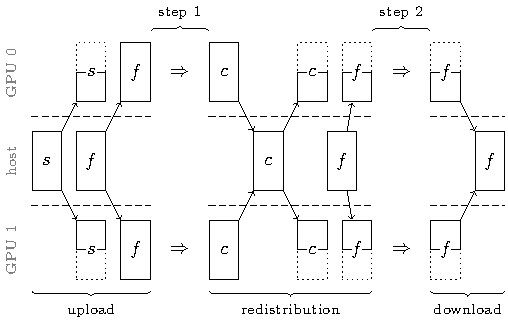
\includegraphics[width=.6\textwidth]{ASHES/lmosem_distribution}
 \caption{Data distribution changes and computations during a single subset iteration of list-mode OSEM using two GPUs.}
 \label{fig:list-mode_OSEM:gpu}
\end{figure*}

\subsubsection{Parallelization strategy}
\label{sec:list-mode_OSEM:strategy}

For parallelization, we consider two possible decomposition strategies for the OSEM algorithm as initially suggested in~\cite{JJK03}: Projection Space Decomposition (PSD) and Image Space Decomposition (ISD).

In PSD, the subsets are split into sub-subsets that are processed simultaneously while all processing units access a common reconstruction and error image.
Using this approach, we are able to parallelize step~1 of the algorithm, but step~2 is performed by a single processing unit.
On a multi-GPU system, we have to copy the reconstruction image to all GPUs before each iteration, and we have to merge all GPUs' error images computed in step~1 before proceeding with step~2.
While both steps are easy to implement, step~2 does not efficiently use the available processing units.

In ISD, the reconstruction image is partitioned, such that each processing unit processes the whole subset with respect to a single part of the reconstruction image.
Thus we are able to parallelize both steps of list-mode OSEM, but each processing unit still accesses the whole reconstruction image in order to compute the error value for each path before merging it with the error image.
On a multi-GPU system, the whole subset has to be copied to each GPU in step~1.
ISD requires large amounts of memory (up to several GB in practically relevant cases) to save all paths computed in step~1.
Summarizing, it is hard to implement step~1 on the GPU, while step~2 can be parallelized easily.

Therefore, we decided to use a hybrid strategy for implementing list-mode OSEM on a multi-GPU system:
Step~1 is parallelized using the PSD approach, while we use ISD for step 2.
This results in the sequence of five phases shown both in Figure~\ref{fig:list-mode_OSEM:gpu} and Listing~\ref{lst:list-mode_OSEM:skelcl}:
\begin{enumerate}
\item \emph{Upload:} the subset ($s$) is divided into sub-subsets, one sub-subset per GPU.
      One sub-subset and the reconstruction image ($f$) are uploaded to each GPU.
\item \emph{Step 1:} each GPU computes a local error image ($c$) for its sub-subset using a map skeleton with additional arguments.
\item \emph{Redistribution:} the local error images that are distributed on all GPUs are downloaded and combined into a single error image on the host by performing element-wise addition.
      Afterwards, the combined error image and reconstruction image are partitioned, in order to switch the parallelization strategy from PSD to ISD.
      The corresponding parts of both images are distributed to the GPUs again.
\item \emph{Step 2:} each GPU updates its part of the reconstruction image using a zip skeleton
\item \emph{Download:} finally, all parts of the reconstruction image are downloaded from the GPUs to the host and merged into a single reconstruction image.
\end{enumerate}

\begin{lstlisting}[%
caption={Parallel implementation of list-mode OSEM in SkelCL.},%
float,%
label={lst:list-mode_OSEM:skelcl},%
numbers=left,%
xleftmargin=2em]
for (l = 0; l < num_subsets; l++) {
  /* 1. Upload: distribute events to devices*/
  Vector<Event> events(read_events());
  events.setDistribution(Distribution::block);
  f.setDistribution(Distribution::copy);
  c.setDistribution(Distribution::copy(add));
  /* 2. Step 1: compute error image
        (map skeleton) */
  mapComputeC(index,events,events.sizes(),f,c);
  c.dataOnDevicesModified();
  /* 3. Redistribution: distribute
        reconstruction image to devices; reduce
        (element-wise add) all error images and
        distribute result to devices */
  f.setDistribution(Distribution::block);
  c.setDistribution(Distribution::block);
  /* 4. Step 2: update reconstruction image
        (zip skeleton) */
  zipUpdate(f, c, f);
  /* 5. Download: merge reconstruction image
        (is performed implicitly) */ }
\end{lstlisting}

The SkelCL program in Listing~\ref{lst:list-mode_OSEM:skelcl} reflects the described five phases in a concise, high-level manner, as shown by the corresponding comments.
The subset, the error image, and the reconstruction image are declared as SkelCL vectors which enables an easy and automatic data transfer between GPUs.
As data transfers are performed implicitly by SkelCL, the upload phase (1.) is implemented by simply setting vector distributions (lines 4--6), while the download phase (5.) is omitted entirely.

\subsubsection{Programming effort: SkelCL vs. OpenCL \& CUDA}
\label{sec:list-mode_OSEM:implementation}

Using the described hybrid parallelization strategy, we developed three parallel implementations of list-mode OSEM using: 1) CUDA, 2) OpenCL, and 3) SkelCL. %~\cite{ScVGM-08}
To study the programming effort, we compare the program sizes in LOC (lines of code).
Though LOC is not a universal measure for programming effort, we consider it as a reasonable first approximation.

We observe~(see Figure~\ref{fig:list-mode_OSEM:LOC}) that while the kernel size in CUDA and OpenCL, or the user-defined function in SkelCL, respectively, are rather similar (about 200 LOC), the lengths of the corresponding host programs differ considerably.
Unlike CUDA, OpenCL requires code for selecting the target platform and an OpenCL device and for compiling kernel functions at runtime.
For a single GPU, the OpenCL-based implementation has the longest code (206 LOC), i.\,e. about 2.5 times longer than the CUDA-based host program (88 LOC) and more than 11 times longer than the SkelCL program.
Our SkelCL-based implementation has 18 LOC, i.\,e. its length is only about 20\% of the CUDA-based version.

Using multiple GPUs in OpenCL and CUDA requires explicit code for additional data transfers between GPUs.
Prior to CUDA 4.0, also multi-threaded code was required to manage several GPUs.
This accounts for additional 42 LOC for the CUDA-based implementation and additional 37 LOC for the OpenCL-based one.
In SkelCL, only 8 additional LOC are necessary to describe the changes of data distribution.
These lines are easily recognizable in the SkelCL program (lines 4--6, 11--12 in Listing~\ref{lst:list-mode_OSEM:skelcl}, plus 3 lines during the initialization) and make this high-level code arguably better understandable and maintainable than the CUDA and OpenCL versions.

\subsubsection{Performance experiments: SkelCL vs. OpenCL \& CUDA}
\label{sec:list-mode_OSEM:runtime}

We evaluated the runtimes of our three implementations of list-mode OSEM, by reconstructing an image of $150\times 150\times 280$ voxels from a real-world PET data set with about $10^8$ events.
From this data set, about $10^2$ equally sized subsets are created.
In our experiments, we measured the average runtime of processing one subset.
In a full reconstruction application, all subsets are processed multiple times, thus making list-mode OSEM a time-intensive application that runs several hours on a single-core CPU.
Unlike CUDA, both OpenCL and SkelCL compile kernels at runtime.
As compilation is only required once, when launching the implementation, but not during the subset iterations, we excluded compilation time from our runtime measurements.
We ran our implementations on a system comprising a quad-core CPU (Intel Xeon E5520, 2.26\,GHz) and an NVIDIA Tesla S1070 system with 4~Tesla GPUs.
Each GPU consists of 240 streaming processors. % running at up to 1.44\,GHz.
The CPU has 12\,GB of main memory, while each GPU owns 4\,GB of dedicated memory.

Figure~\ref{fig:list-mode_OSEM:runtime} shows the runtime of our three implementations of list-mode OSEM using up to four GPUs.
We observe that CUDA always provides best performance, being about 20\% faster than OpenCL and SkelCL on the same number of GPUs.
As compared to the OpenCL-based implementation, SkelCL introduces only a moderate overhead of less than 5\%.
Hence, the runtime overhead of SkelCL as compared to CUDA is mainly caused by the fact that SkelCL is built on top of OpenCL.

\begin{figure}[tb]
  \centering
  \begin{subfigure}{.45\textwidth}
    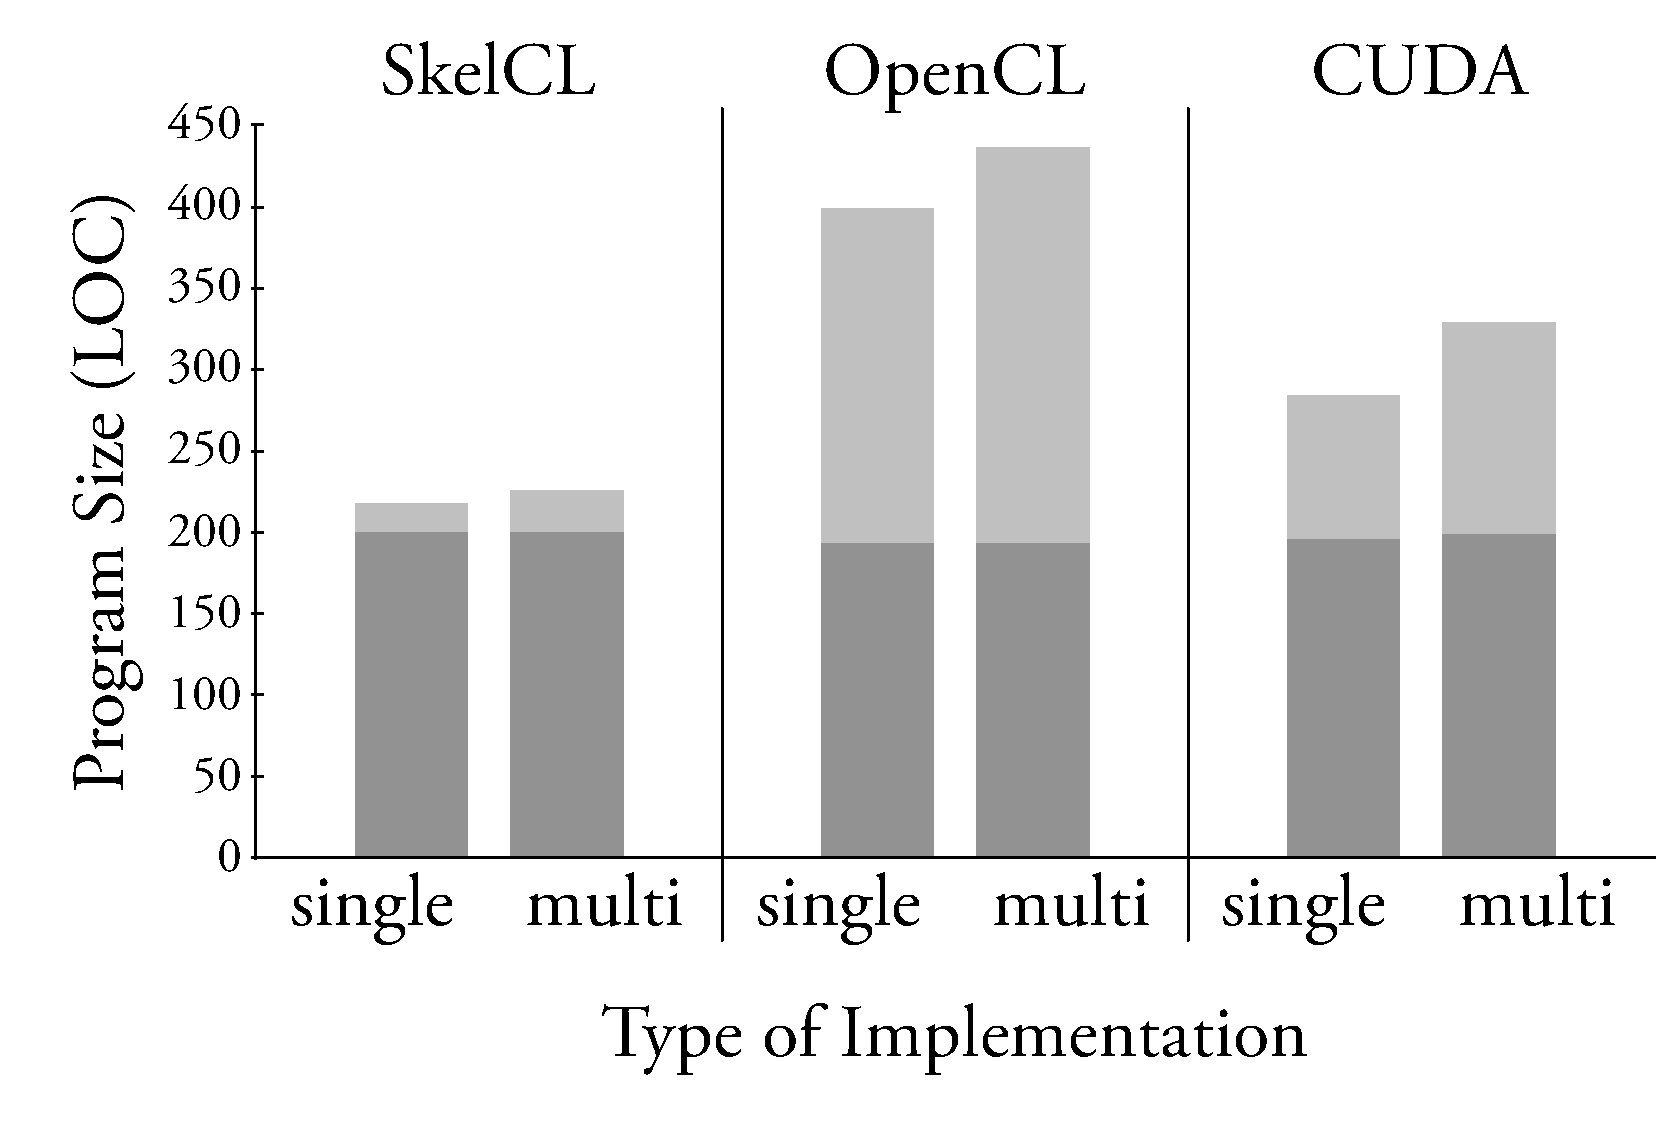
\includegraphics[width=\textwidth]{ASHES/loc}
    \caption{Lines of code for host (light gray) and GPU (dark gray)}
    \label{fig:list-mode_OSEM:LOC}
  \end{subfigure}
  \hfill
  \begin{subfigure}{.45\textwidth}
    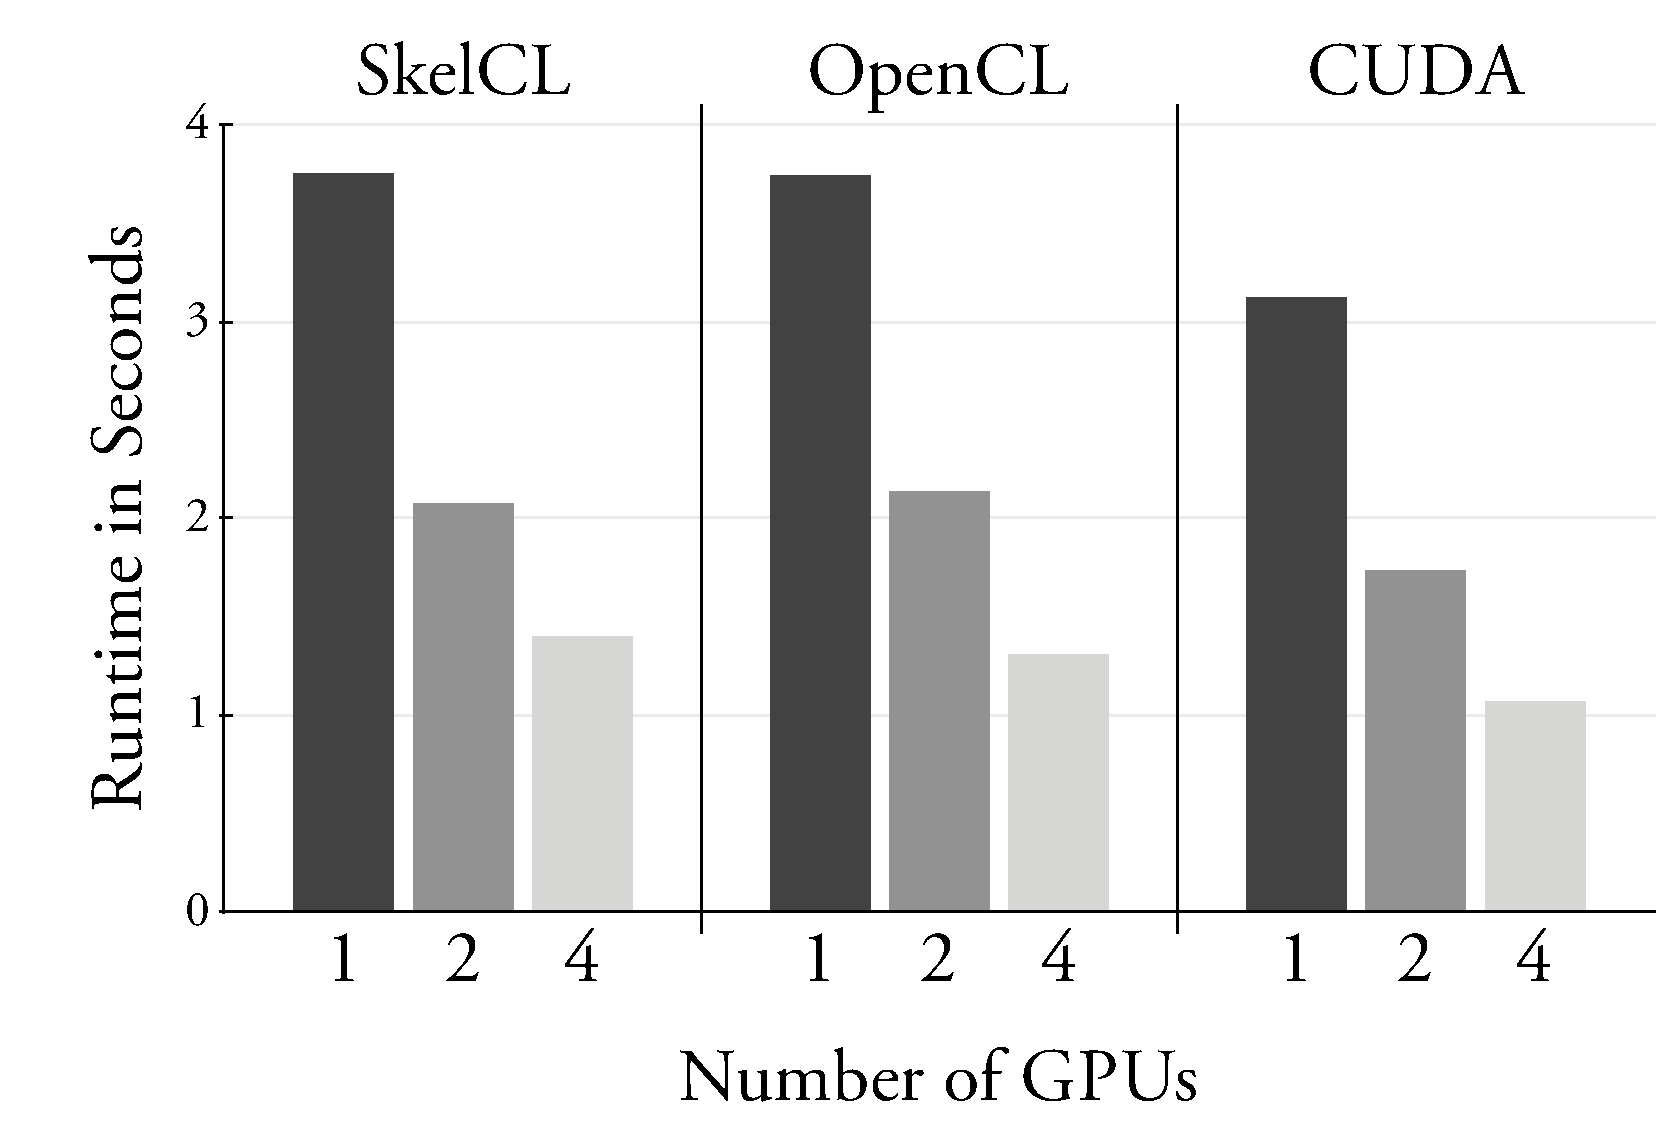
\includegraphics[width=\textwidth]{ASHES/lmosemIteration}
    \caption{Average runtime of one subset iteration}
    \label{fig:list-mode_OSEM:runtime}
  \end{subfigure}
  \caption{Program size of parallel list-mode OSEM (single- and multi-GPU versions), and runtime for processing one subset using SkelCL, OpenCL, and CUDA.}
  \label{fig:list-mode_OSEM:results}
  \bigskip
\end{figure}
\from{ASHES end}

\from{ICCS begin}
\subsection{Iterative PET Image Reconstruction and the LM OSEM Algorithm (ICCS)}
% \label{sec:pet}
% Our running application example in this paper is the LM OSEM algorithm~\cite{READER, sgmkswb09} for image reconstruction used in Positron Emission Tomography (PET).
% In PET, a radioactive substance is injected into a human or animal body, which is then placed inside a PET scanner that contains several arrays of detectors.
% As the particles of the applied substance decay, positrons are emitted (hence the name PET) and annihilate with nearby electrons, such that two photons are emitted in the opposite directions (see Fig.~\ref{fig:scanner and detector}).
% These ``decay events'' are registered by two opposite detectors of the scanner which records these events in a list.
% Data collected by the PET scanner are then processed by a reconstruction algorithm to obtain a resulting image.

% \begin{figure}
% \centering
% 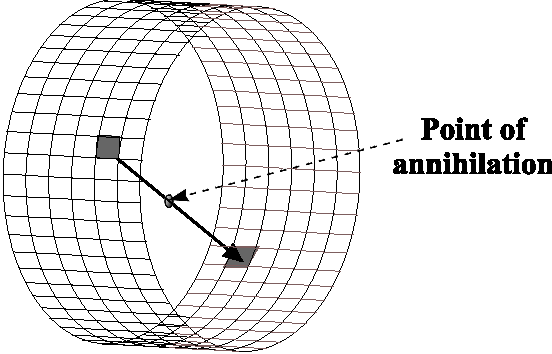
\includegraphics[scale=0.50]{ICCS/ringscanner}
% \caption{Two detectors register an event in a PET-scanner}
% \label{fig:scanner and detector}
% \end{figure}

% \subsubsection{The LM OSEM Algorithm}
% List-Mode Ordered Subset Expectation Maximization \cite{READER} (called LM OSEM in the sequel) is a block-iterative algorithm for 3D image reconstruction.
% LM OSEM takes a set of events from a PET scanner and splits them into $s$ equally sized subsets.
% Then, for each subset $S_l, l \in {0, \ldots, s-1}$, the following computation is performed:
% \begin{equation}
% f_{l+1}=f_{l}c_{l};\quad
% c_{l}=\dfrac{1}{A_N^T \textbf{1}}
% \sum_{i \in S_{l}} (A_i)^T \dfrac{1}{A_{i} f_{l}}.
% \label{equ:lm_osem}
% \end{equation}

% Here $f \in \mathbb{R}^n$ is a 3D image in vector form with dimensions $n = (X \times Y \times Z)$, $A$ -- the so called system matrix, element $a_{ik}$ of row $A_i$ is the length of intersection of the line between the two detectors of event $i$ with voxel $k$ of the reconstruction image, computed with Siddon's algorithm \cite{SIDDON}.
% $\dfrac{1}{A_N^T \textbf{1}}$ is the so-called normalization vector; since it can be precomputed, we will omit it in the following.
% The multiplication $f_{l}c_{l}$ is performed element-wise.
% Each subset's computation takes its predecessor's output image as input and produces a new, more precise image.

% The structure of a sequential LM OSEM implementation is shown in Listing~\ref{lst:seq_code}.
% The outermost loop iterates over the subsets.
% The first inner loop (step 1) iterates over subset's events to compute $c_l$, which requires three sub-steps:
% row $A_i$ is computed from the current event using Siddon's algorithm;
% the local error for row $A_i$ is computed and, finally, added to $c_l$.
% The second inner loop (step 2) iterates over all elements of $f_l$ and $c_l$ to compute $f_{l+1}$.
% \begin{figure}
% \begin{lstlisting}[caption={Sequential code for LM OSEM comprises one outer loop with two nested inner loops.},label={lst:seq_code}]
% for (int l = 0; l < subsets; l++) {
%   /* read subset */

%   /* step 1: compute error image c_l */
%   for (int i = 0; i < subset_size; i++) {
%     /* compute A_i            */
%     /* compute local error    */
%     /* add local error to c_l */  }

%   /* step 2: update image estimate f */
%   for (int k = 0 ; k < image_size; k++) {
%     if (c_l[k] > 0.0) { f[k] = f[k] * c_l[k]; } }  }
% \end{lstlisting}
% \end{figure}

% \subsubsection{Parallelization of LM OSEM in OpenCL}
% \label{sec:parallel_implementation}
% LM OSEM is a rather time-consuming algorithm that needs parallelization:
% a typical 3D image reconstruction processing $6 \cdot 10^7$ input events for a $150 \times 150 \times 280$ PET image takes more than two hours on a modern PC.

% Although the iterations of the outer loop in Listing~\ref{lst:seq_code} are inherently sequential,
% we can parallelize the two calculation steps within one iteration as shown in Fig.~\ref{fig:em_distribution} for a system comprising one CPU and two GPUs.
% Note that these steps require different data distribution patterns:
% \begin{itemize}
%   \item[] \emph{Step 1:} Subset's events are copied from the CPU to all GPUs (\emph{upload}) to compute the summation part of $c_l$ concurrently. This step requires that the complete image estimate $f_l$ is available to all GPUs.
%   \item[] \emph{Step 2:} For computing the next image estimate $f_{l+1}$ in parallel, the current image estimate $f_l$ and the error image $c_l$ computed in step 1 have to be distributed in disjoint parts (blocks) among all GPUs.
% \end{itemize}
% \begin{figure}
% \centering
% 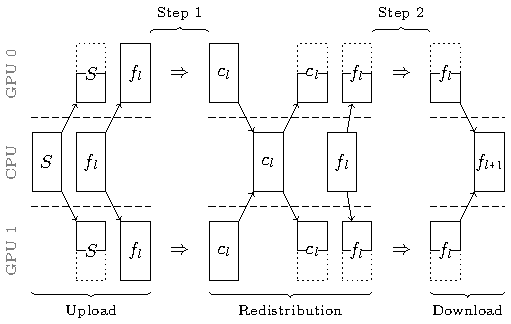
\includegraphics[width=0.6\textwidth]{ICCS/em_distribution}
% \caption{Parallelization schema of the LM OSEM algorithm.}
% \label{fig:em_distribution}
% \end{figure}
% Thus, the parallelization schema in Fig.~\ref{fig:em_distribution} requires a data \emph{redistribution} phase between the two computation steps.
% During step 1, each GPU computes a partial sum of $c_l$.
% After step 1, all partial results are summed up and redistributed disjointly to all GPUs.
% Note that for step 1, each GPU requires a full copy of the image estimate, while in step 2 all GPUs update disjoint parts of it.
% After step 2, the disjoint parts of the image estimate are copied from all GPUs back to the CPU (\emph{download}).

% \bigskip\noindent
% In the following, we describe how the parallelization schema phases in Fig.~\ref{fig:em_distribution} are implemented using OpenCL.

% \paragraph{Upload}
% The simplified OpenCL implementation of the upload phase is shown in Listing~\ref{lst:upload}.
% Uploading of the event vector $S$ is performed in lines 3--6, while lines 9--12 show the upload of the image estimate $f_l$.
% In OpenCL, we have to manage each GPU explicitly, therefore, for each GPU, we create a set of buffers (\texttt{s\_gpu} and \texttt{f\_gpu}) and we use a loop (line 1) to repeat all memory operations for each GPU.
% For performance reasons, we use asynchronous copy operations, specified using the \texttt{CL\_FALSE} flag (line 3 and 9): this allows data transfers to multiple GPUs to overlap.
% We perform different operations with $S$ (distribute among all GPUs) and $f_l$ (copy to each GPU), therefore, there are differences when specifying the amount of bytes to copy (lines 4 and 10) and the offsets in the CPU memory (lines 5 and 11).
% Altogether eleven such memory operations -- each with different amounts and offsets -- appear in the OpenCL source code.

% \begin{lstlisting}[caption={Implementation of the upload phase in OpenCL (ommitting error checks for brevity)},label={lst:upload},numbers=left]
% for (int gpu = 0; gpu < gpu_count; gpu++) {
%   // upload $S$
%   clEnqueueWriteBuffer( command_queue[gpu], s_gpu[gpu], CL_FALSE, 0,
%                         sizeof(float) * size_of_s / gpu_count,
%                         (void*)&s_cpu[ gpu * size_of_s / gpu_count ],
%                         0, NULL, NULL );

%   // upload $f_l$
%   clEnqueueWriteBuffer( command_queue[gpu], f_gpu[gpu], CL_FALSE, 0,
%                         sizeof(float) * size_of_f,
%                         (void*)&f_cpu[0],
%                         0, NULL, NULL ); }
% \end{lstlisting}

% \paragraph{Step 1}
% The implementation of step 1 performs the operations shown in Listing~\ref{lst:seq_code}: first computing $A_i$, then the local error for $A_i$ and finally adding the local error to $c_l$.
% Because of GPU memory restrictions, the OpenCL implementation is not straightforward, such that, for the sake of brevity, we will not discuss it in more detail here.

% \paragraph{Redistribution}
% Listing~\ref{lst:redistribution} shows an OpenCL pseudocode for the redistribution phase.
% To download the data from all GPUs, we use the \texttt{clEnqueueReadBuffer} function and perform the operations asynchronously, but this time, we have to wait for the operations to finish.
% For such synchronization, OpenCL uses \emph{events}, associated with an operation (line 3) for waiting for the operation to finish (line 4).
% After all downloads have finished, we combine the different values of $c_l$ to a new value of $c_l$ on the CPU (line 7), and upload the blocks of $c_l$ to the GPUs.
% Even if we only copied data between GPUs, without processing them on the CPU, we still would have to download them to the CPU because direct GPU-to-GPU transfers are currently not possible in OpenCL.

% \begin{lstlisting}[caption={OpenCL pseudocode for the redistribution phase},label={lst:redistribution},numbers=left]
% // download all c_l values from the GPUs to the CPU
% cl_event events[gpu_count];
% for (int gpu = 0; gpu < gpu_count; gpu++) { clEnqueueReadBuffer( ..., &events[gpu] ); }
% clWaitForEvents(gpu_count, events);

% // combine data on CPU
% combine( ... );

% // upload block of the new c_l version to each GPU
% for (int gpu = 0; gpu < gpu_count; gpu++) { clEnqueueWriteBuffer( ... ); }
% \end{lstlisting}

% \paragraph{Step 2}
% Listing~\ref{lst:step_2} shows the implementation of step 2.
% In OpenCL, computations are specified as \emph{kernels} which are created from the source code specifying the computation.
% The computation in step 2 is, therefore, described as a string in lines 3 -- 5.
% The operations used here are the same as in the sequential code in Listing~\ref{lst:seq_code}.

% For executing the computations of step 2, we have to perform the following steps for each GPU:
% \begin{itemize}
%   \item create an OpenCL kernel from the source code (requires 50 lines of code in OpenCL);
%   \item compile the kernel specifically for the GPU (requires 13 lines of code in OpenCL);
%   \item specify kernel arguments one-by-one using the \texttt{clSetKernelArg} function (line 12 -- 17);
%   \item specify execution environment, i.\,e., how many instances of the kernel to start (line 20 -- 21);
%   \item launch the kernel (line 23 -- 24).
% \end{itemize}
% \begin{lstlisting}[caption={Implementation of step 2 in OpenCL (omitting error checks for brevity)},numbers=left,label={lst:step_2}]
% // step 2 (in Fig. 2)
% source_code_step_2 =
% "__kernel void step2(__global float* f, __global float* c_l, int offset, int size) { \
%   int id = get_global_id(0) + offset;                                                \
%   if (id < size && c_l[id] > 0.0) { f[id] = f[id] * c_l[id]; } }";

% for (int gpu = 0; gpu < gpu_count; gpu++) {
%  // create kernel (50 lines of code)
%  // compile kernel (13 lines of code)

%  // specifying kernel arguments:
%   clSetKernelArg(kernel_step2[gpu], 0, sizeof(cl_mem), (void*)&f_buffer[gpu]);
%   clSetKernelArg(kernel_step2[gpu], 1, sizeof(cl_mem), (void*)&c_l_buffer[gpu]);
%   int offset = gpu * (size_of_f / gpu_count);
%   clSetKernelArg(kernel_step2[gpu], 2, sizeof(int), (void*)&offset);
%   int size   = MIN( (gpu + 1) * (size_of_f / gpu_count), size_of_f );
%   clSetKernelArg(kernel_step2[gpu], 3, sizeof(int), (void*)&size);

%  // specify execution environment
%   int local_work_size[1]  = { 32 };
%   int global_work_size[1] = { roundUp(32, size_of_f / gpu_count) };
%  // launch the kernel
%   clEnqueueNDRangeKernel(command_queue[gpu], kernel_step2[gpu],
%                          1, NULL, &global_work_size, &local_work_size, 0, NULL, NULL); }
% \end{lstlisting}


% \paragraph{Download}
% The implementation of the download phase is similar to the upload phase (Listing~\ref{lst:upload}).
\from{ICCS end}

\from{ICCS begin}
\subsection{Implementing the LM OSEM Algorithm using SkelCL (ICCS)}
\label{sec:experiments}
\label{sec:experiments:skelcl}
We assess the programming effort and runtime performance of our approach by comparing the SkelCL implementation of the LM OSEM algorithm against its OpenCL implementation.

\paragraph{Programming effort}

The parallel SkelCL code in Listing~\ref{lst:em_skelcl} fully retains the original sequential structure of Listing~\ref{lst:seq_code}, which makes it well structured and easily understandable.
\begin{lstlisting}[%
  caption={SkelCL code of the LM OSEM algorithm},%
  numbers=left,%
float,%
label={lst:em_skelcl}]
Map<void(int)> computeC_l("void func(int index, event* s, float* f, float* c_l) {   \
  for (int i = index; i < subset_size; i+=512) {                                    \
    // compute A_i // compute local error // add local error to c_l                 \
  } }");
Zip<float(float, float)> updateF("float func(float f_i, float cl_i) {               \
      if (cl_i > 0.0) return f_i * cl_i; else return f_i; }");

Vector<float> f   = readStartImage();
Vector<int> index = createIndexVector(512);
for (i = 0; i < num_iterations; ++i) {
  Vector<event> s = read_subset(); // read subset s from file
  Vector<float> c_l(image_size);
  s.setDistribution(block);
  f.setDistribution(copy);
  c_l.setDistribution(copy, add);

  /* step 1. compute error image c_l */
  computeC_l(index, s, f, c_l);

  f.setDistribution(block);
  c_l.setDistribution(block);

  /* step 2. update image estimate f */
  f = updateF(f, c_l); }
\end{lstlisting}
The sequential loops are replaced by skeleton calls (line 18 and 24) which take the code from the corresponding loop's body, and only 5 lines of code are added for data distribution (lines 13 -- 15 and 20 -- 21).
The computation of the error image is expressed using a map skeleton (lines 1 -- 4).
Due to memory restrictions, it is not possible to apply the map skeleton to the whole vector \texttt{s}:
map is rather applied to a vector of size 512 (line 9), such that for every index a block of elements is processed using the loop in line 2.
Since detecting memory restrictions and applying blocking automatically is non-trivial, SkelCL currently relies on the user to resolve such situations.
The event vector, the image estimate, and the error image are passed as additional arguments to the skeleton.
The zip skeleton is used for updating the error image (line 5 -- 6).

The SkelCL-based implementation of the LM OSEM is considerably shorter than the OpenCL code:
with 232 lines of code (customizing functions: 200~lines, host program: 32~lines) as compared to 436 lines of code (kernel functions: 193~lines, host program: 243~lines) in the OpenCL-based implementation; we save almost 50\% of the lines of code.
When using SkelCL, we do not have to implement the tedious and lengthy initialization of OpenCL.
Expressing the computations as skeletons liberates us from dealing with pointers in the kernel and repeatedly performing the same sequence of steps for each computation.
By using container data types, we avoid additional programming effort to implement data transfers between CPU and GPU or between multiple GPUs, and we obtain a multi-GPU-ready implementation of LM OSEM for free.


\paragraph{Runtime performance}
We tested the performance of our implementations using an NVIDIA Tesla S1070 system comprising 4 Tesla GPUs.
Each GPU consists of 240 streaming processors.

Fig.~\ref{fig:lmosem_runtime} compares the runtime of one iteration for our SkelCL and OpenCL implementations using one, two, and four GPUs, correspondingly.
While the differences in the programming effort to implement the two versions are significant, the differences in runtime are very small.
When running on a single GPU, both implementations take the same time (3.66 seconds) to complete.
With two and four GPUs, the OpenCL implementation slightly outperforms the SkelCL implementation, being 1.2\% and 4.7\% faster.
We presume that the increasing overhead is caused by the more complex data distribution performed when using more GPUs.
Comparing to the significant reduction in programming effort (50\%), the runtime overhead of less than 5\% is arguably a moderate one.
\vfill
\begin{figure}
  \centering
  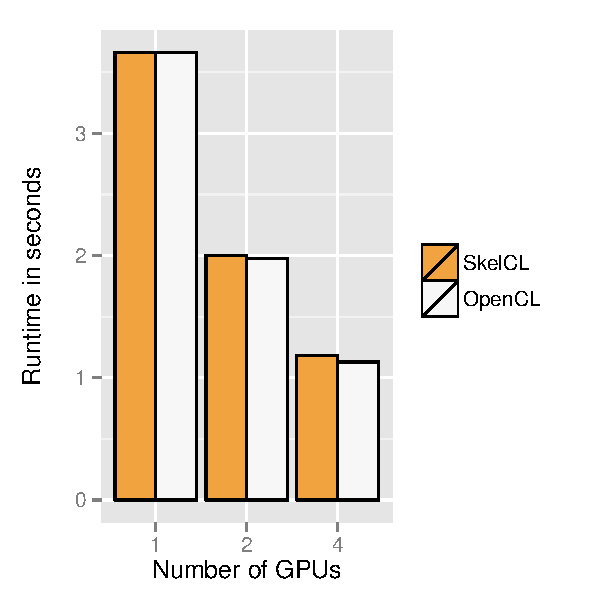
\includegraphics[width=.4\textwidth]{ICCS/skelcl-runtime.pdf}
  \caption{Average runtime of one iteration of the LM OSEM algorithm using SkelCL and OpenCL.}
  \label{fig:lmosem_runtime}
\end{figure}
\from{ICCS end}

